\chapter{Stage 1 --- Cornea-Plane Diffraction}
\label{ch:stage1}

\section{Scope and purpose}

Stage 1 (\texttt{stage1\_v2/}) is the project's earliest and most narrowly-scoped
module: it propagates a circular pinhole's field via the exact ASM
(Section~\ref{ch:wave_optics}) from the pinhole plane to the corneal plane only. It
deliberately never touches the eye lens, vitreous, retina, or image formation, and
never estimates a single ``best'' pinhole --- it only characterizes the field at one
intermediate plane, as an independently checkable building block for Stage 2.

\section{Validation}

Stage 1 is validated against real closed-form theory: the Fresnel on-axis intensity
oscillation formula
\begin{equation}
I(0,z) = 4 I_0 \sin^2\!\left(\frac{\pi N_F}{2}\right)
\end{equation}
which predicts on-axis intensity oscillates with propagation distance as the Fresnel
number $N_F$ passes through successive half-integers --- a genuine near-field effect,
not an artifact. Stage 1's numerical on-axis intensity vs.\ distance matches this
closed form at $r=0.997$ correlation.

\section{Full sweep}

Table~\ref{tab:stage1-full} reports one representative slice of this report's Stage 1
sweep (fixed $12\mm$ gap, $550\,$nm) across the full 15-aperture grid --- this stage has
no myopia ($M$) dependence, since it stops before the eye lens. Figure~\ref{fig:stage1-ee}
shows all four effective-radius definitions (Section~\ref{sec:effective-radius}) as a
function of aperture at the corneal plane.

\begin{figure}[htbp]
\centering
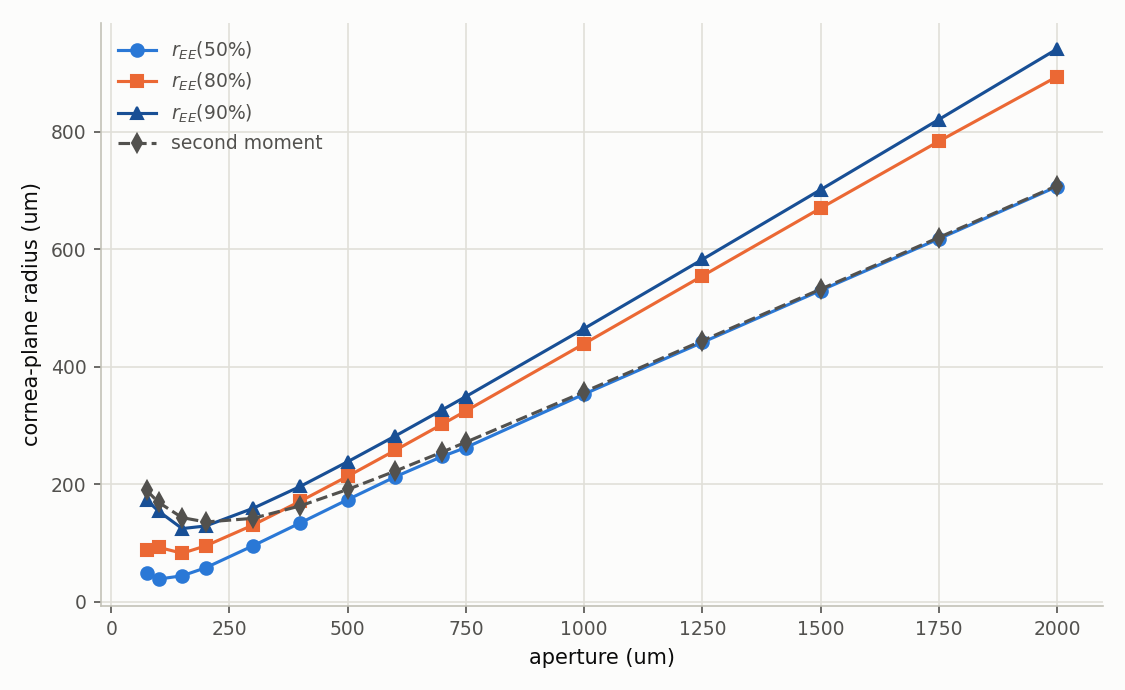
\includegraphics[width=0.85\textwidth]{figures/fig_stage1_cornea_radii.png}
\caption{Stage 1: cornea-plane effective radii ($r_{EE}(50\%)$, $r_{EE}(80\%)$,
$r_{EE}(90\%)$, second-moment radius) vs.\ pinhole aperture, $12\mm$ gap, $550\,$nm.}
\label{fig:stage1-ee}
\end{figure}

{\small
\begin{longtable}{rrrrrrr}
\caption{Stage 1 cornea-plane sweep, 12mm gap, 550nm.}\label{tab:stage1-full}\\
\toprule
a\_hole (um) & N\_F & regime & r\_EE50 (um) & r\_EE80 (um) & r\_EE90 (um) & 2nd moment (um) \\
\midrule
\endfirsthead
\multicolumn{7}{c}{\tablename\ \thetable\ -- continued}\\
\toprule
a\_hole (um) & N\_F & regime & r\_EE50 (um) & r\_EE80 (um) & r\_EE90 (um) & 2nd moment (um) \\
\midrule
\endhead
\bottomrule
\endfoot
75 & 0.21 & Transition & 48.55 & 87.78 & 173.48 & 189.66 \\
100 & 0.38 & Transition & 38.90 & 92.94 & 154.46 & 169.45 \\
150 & 0.85 & Transition & 44.48 & 82.87 & 124.81 & 143.45 \\
200 & 1.52 & Transition & 58.22 & 95.45 & 129.27 & 136.03 \\
300 & 3.41 & Transition & 95.59 & 130.87 & 159.29 & 142.23 \\
400 & 6.06 & Transition & 134.52 & 171.46 & 196.64 & 163.51 \\
500 & 9.47 & Transition & 174.04 & 213.75 & 238.54 & 191.35 \\
600 & 13.64 & Strong Fresnel & 212.67 & 257.74 & 282.05 & 222.39 \\
700 & 18.56 & Strong Fresnel & 247.50 & 302.38 & 326.82 & 255.08 \\
750 & 21.31 & Strong Fresnel & 262.67 & 324.88 & 349.42 & 271.75 \\
1000 & 37.88 & Strong Fresnel & 353.54 & 439.26 & 465.06 & 357.36 \\
1250 & 59.19 & Strong Fresnel & 441.50 & 554.48 & 582.55 & 444.35 \\
1500 & 85.23 & Strong Fresnel & 529.79 & 669.73 & 701.18 & 531.98 \\
1750 & 116.00 & Strong Fresnel & 617.61 & 783.54 & 820.59 & 619.95 \\
2000 & 151.52 & Strong Fresnel & 706.59 & 893.56 & 940.60 & 708.10 \\
\end{longtable}
}

\textbf{Reading this chapter's results}: cornea-plane blur is monotonically decreasing
with aperture over most of this range (a larger pinhole diffracts less), the opposite
trend from the retina-plane result in Chapter~\ref{ch:stage2} once the eye's own
converging lens and myopic defocus are added --- the retina-plane optimum exists
precisely \emph{because} those two effects (diffraction favoring large apertures,
defocus favoring small ones) trade off against each other, a genuine competition Stage
1 alone cannot show since it stops before the lens.
